\section{Results}

To test the clustering algorithm, a terrain is loaded, it's resources edited and five clusters produced. These clusters are subsequently analysed to ensure they successfully detect distinct resource features on which to cluster.\\

The terrain used is a model of the Grand Canyon using data from the US Geological Survey \protect\footnotemark \footnotetext{\url{http://www.usgs.gov}}. This terrain is chosen as its canyons and crevasses make ground illumination vary greatly.\\

The following resource edits were performed on the terrain:

\begin{itemize}
\item \textit{Latitude}: Set to zero degrees (equator)
\item \textit{Soil Infiltration}: 5 millimetres for all terrain points with a slope under 30 degrees. All points with a slope over 30 degrees were set to 0 to simulate a cliff.
\item \textit{Rainfall}: 25 millimetres for every month.
\item \textit{Temperature}: 15 degrees at 0 meters in December. 30 degrees at 0 metres in June. 
\end{itemize}

The resulting terrain clusters that form are displayed in figure \ref{fig:clustering_test_resulting_clusters} and summarized in appendix \ref{AppendixA}.

\begin{figure}
\center
	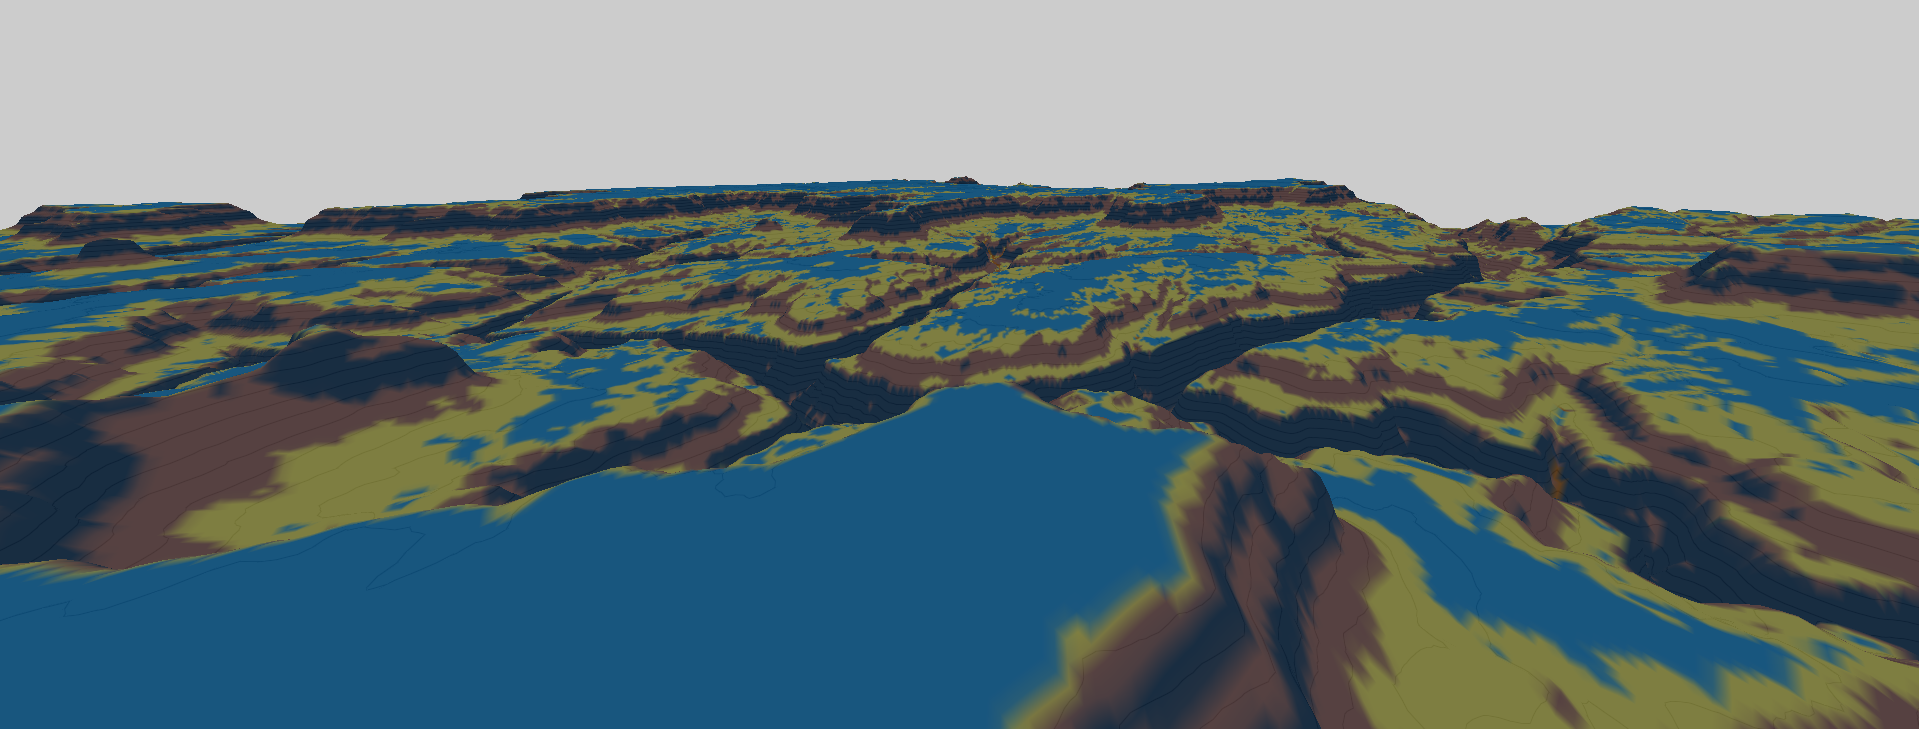
\includegraphics[width=\textwidth]{clustering_test_resulting_clusters.png}
	\caption{ Clustering test: Resulting terrain clusters}	
	\label{fig:clustering_test_resulting_clusters}
\end{figure}

\definecolor{cluster_1}{rgb}{0.8,0.4,0.0}
\definecolor{cluster_2}{rgb}{0.6,0.4,0.4}
\definecolor{cluster_3}{rgb}{0.0,0.2,0.4}
\definecolor{cluster_4}{rgb}{1.0,1.0,0.4}
\definecolor{cluster_5}{rgb}{0.0,0.6,1.0}

\begin{figure}
\center
	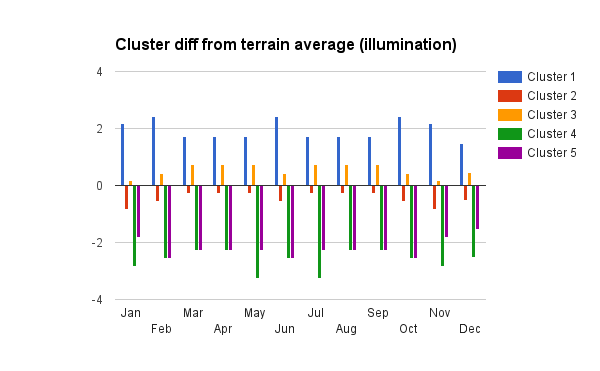
\includegraphics[width=\textwidth]{clustering_graph_illumination_diff.png}
	\caption{ Monthly illumination for each cluster and the average over the whole terrain.}	
	\label{fig:clustering_graph_illumination}
\end{figure}

\begin{figure}
\center
	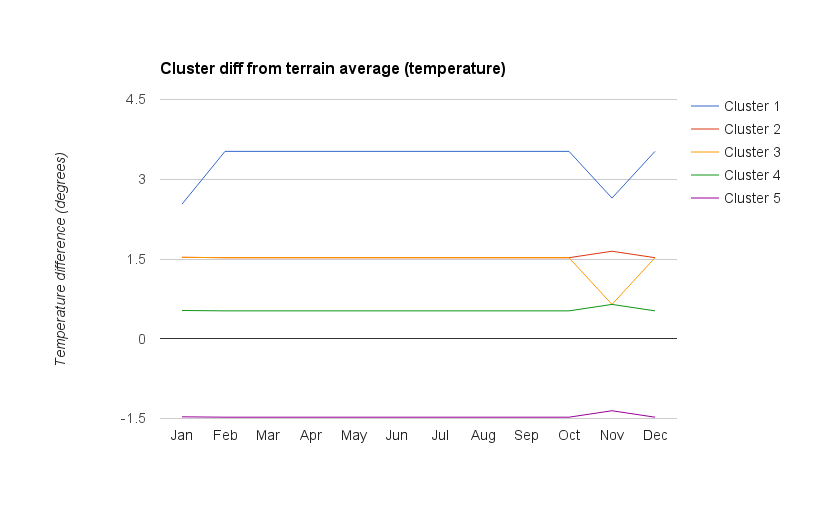
\includegraphics[width=\textwidth]{clustering_graph_temp_diff.png}
	\caption{ Monthly temperature for each cluster and the average over the whole terrain. Cluster 2 has the same values as cluster 4.}	
	\label{fig:clustering_graph_temp}
\end{figure}

\begin{figure}
\center
	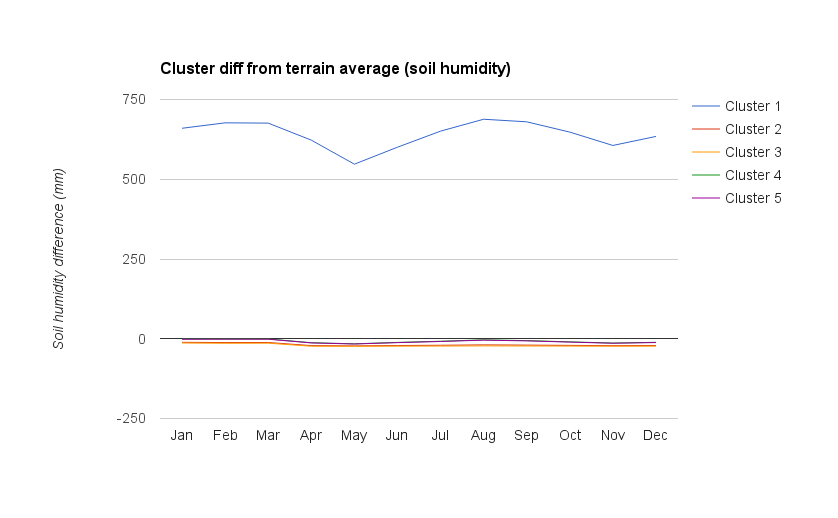
\includegraphics[width=\textwidth]{clustering_graph_soil_humidity_diff.png}
	\caption{ Soil humidity for each cluster (same for every month) and the average over the whole terrain.}	
	\label{fig:clustering_graph_humidity}
\end{figure}

\begin{figure}
\center
	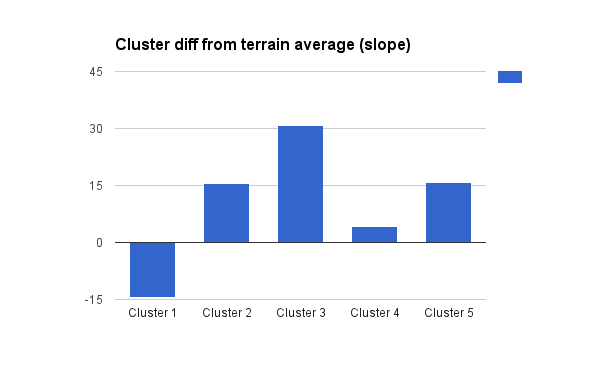
\includegraphics[width=\textwidth]{clustering_graph_slope_diff.png}
	\caption{ Slope for each cluster and the average over the whole terrain.}	
	\label{fig:clustering_graph_slope}
\end{figure}

Figures \ref{fig:clustering_graph_illumination}, \ref{fig:clustering_graph_temp}, \ref{fig:clustering_graph_humidity} and \ref{fig:clustering_graph_slope} show how much each cluster's illumination, temperature, soil humidity and slope vary from the terrain's average. Using this, is is possible to determine the key feature(s) of each individual cluster (summarized in table \ref{tab:clustering_test_cluster_variance}).

\begin{table}[]
  \centering
	    \begin{tabular}{|p{3cm}|p{3cm}|p{3cm}|p{3cm}|p{3cm}|}
		\hline	
  	    \textbf{Cluster} &  \textbf{Illumination} & \textbf{Temperature} & \textbf{Soil Humidity} & \textbf{Slope} \\
		\hline
		\textbf{1} & \textuparrow & \textdownarrow & \textrightarrow & \textdownarrow \textdownarrow \\
		\hline
		\textbf{2} & \textrightarrow & \textuparrow & \textrightarrow & \textuparrow \\
		\hline
		\textbf{3} & \textrightarrow & \textrightarrow & \textrightarrow & \textuparrow \textuparrow \textuparrow \\
		\hline
		\textbf{4} & \textdownarrow \textdownarrow & \textuparrow \textuparrow & \textuparrow \textuparrow \textuparrow & \textrightarrow \\
		\hline
		\textbf{5} & \textdownarrow & \textuparrow & \textdownarrow \textdownarrow & \textuparrow \\
		\hline
		\end{tabular}
		\caption{Summary of cluster feature variance from terrain average.}
	  \label{tab:clustering_test_cluster_variance}
\end{table}